\documentclass[../report.tex]{subfiles}

\begin{document}
\par Étudions dans un premier temps les données selon une approche "série temporelle".

\subsection{Décomposition de la série}

\par On commence par décomposer la série selon un trend et une saisonnalité. Pour cela, plusieurs méthodes s’offrent à nous. Nous choisirons dans un premier temps la méthode de Buys-Ballot généralisée, qui consiste à écrire chacune des composantes déterministes comme une combinaison linéaire de fonctions connues du temps.

\par On obtient alors la décomposition suivante :
\begin{figure}[H]
  \centering
    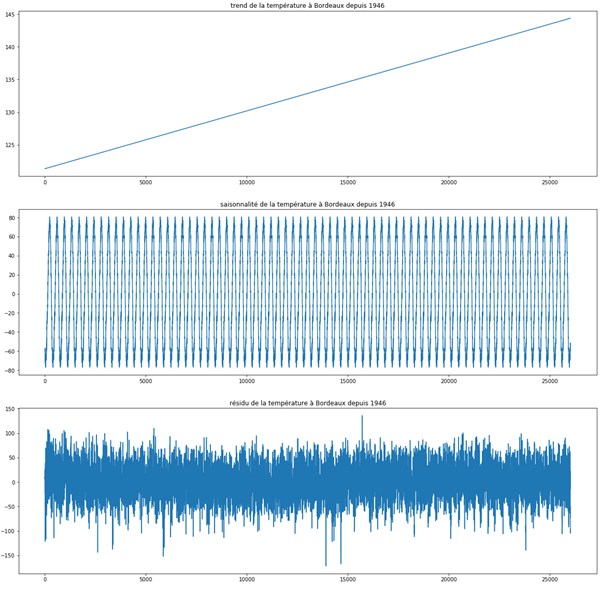
\includegraphics[width=0.7\textwidth]{images/part_1/buysballot.png}
\end{figure}

\par La variance des résidus est élevée en comparaison de la différence du trend entre le début et la fin de la série temporelle ; les données sont fortement bruitées.

\par On aurait également pu envisager une décomposition de la forme Seasonal decomposition of Time series by Loess, ce qui est aisé avec R. On choisit une fenêtre de la largeur d’une période et l’on obtient la décomposition suivante :
\begin{figure}[H]
  \centering
    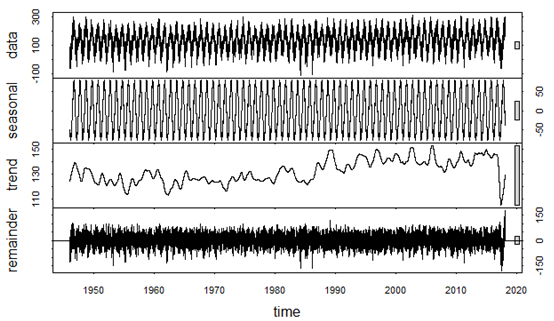
\includegraphics[width=0.7\textwidth]{images/part_1/slt.png}
\end{figure}

\par On obtient pour cette décomposition un écart type de 33,7, à comparer avec le 33,5 de la méthode de Buys-Ballot.

\subsection{Interrogation sur la période de la série}

\par On s’interroge alors sur un point. On sait qu’une année dure 365,24 jours et non pas 365 comme on en fait souvent l’approximation. On a ici pris en compte le décalage dans la formule des Ŝ, mais qu’en serait-il si on l’omettait ? 

\par En refaisant une simulation qui fait cette approximation, on obtient une variance de 33,8 sur les résidus, contre 33,5 dans le cas plus rigoureux. Par la suite on se permettra de désigner la période par 365 ou 365,24 compte tenu de la proximité des deux valeurs.

\subsection{Validité du modèle additif}

\par On a jusque alors envisagé un modèle de type additif pour la série temporelle : la valeur temporelle s’écrirait comme la somme d’une tendance, d’une saisonnalité et d’une erreur que l’on suppose modélisable par un bruit gaussien faible. On va chercher à vérifier cette hypothèse d’additivité en traçant la courbe de l’erreur obtenue (en valeur absolue) en fonction de la valeur prédite par Buys-Ballot généralisé.

\begin{figure}[H]
  \centering
    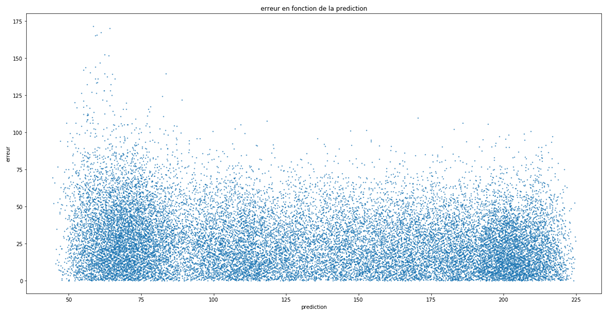
\includegraphics[width=0.7\textwidth]{images/part_1/erreurfpred.png}
\end{figure}

\par On ne distingue pas de relation nette entre la variance du bruit et la grandeur de la prédiction ; aussi le modèle additif sera-t-il considéré comme pertinent par la suite.

\subsection{Modélisation}

\par La présence d’une tendance et d’une saisonnalité nous invite à envisager la modélisation de la série temporelle par un processus de type SARIMA.

\subsection{Ordre de différentiation}

\par Par acquis de conscience, examinons la fonction d’autocorrélation afin de déterminer l’ordre de différentiation requis.

\begin{figure}[H]
  \centering
    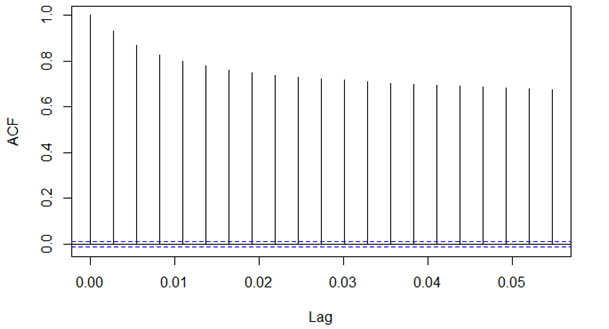
\includegraphics[width=0.7\textwidth]{images/part_1/autocorr1.png}
\end{figure}

\par Comme présumé, le processus est non-stationnaire. On va alors tracer l’autocorrélogramme de la série temporelle différentiée. 

\begin{figure}[H]
  \centering
    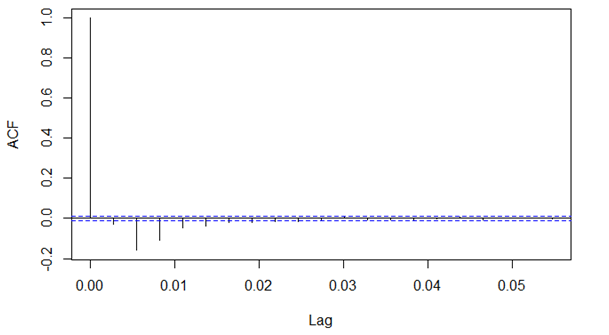
\includegraphics[width=0.7\textwidth]{images/part_1/autocorr2.png}
\end{figure}

\par Cet autocorrélogramme nous invite à considérer qu’un ordre de différentiation 1 est suffisant pour le modèle SARIMA, ce qui concorde avec les décompositions que l’on a obtenu précédemment (les restes ne semblaient pas présenter de tendance quadratique.)

\subsection{Saisonnalité}

\par Les études précédentes et le bon sens climatique nous invitent à considérer une saisonnalité d’ordre 365.

\subsection{Étude des ordres p et q}

\par Un processus AR d’ordre $p$ se caractérise par sa fonction d’autocorrélation partielle qui s’annule à partir de l’ordre $p$ + 1, et un processus MA d’ordre $q$ se caractérise par sa fonction d’autocorrélation qui s’annule à partir de l’ordre $q + 1$.

\par Traçons donc les autocorrélogramme et autocorrélogramme partiel de la série différentiée.

\begin{figure}[H]
  \centering
    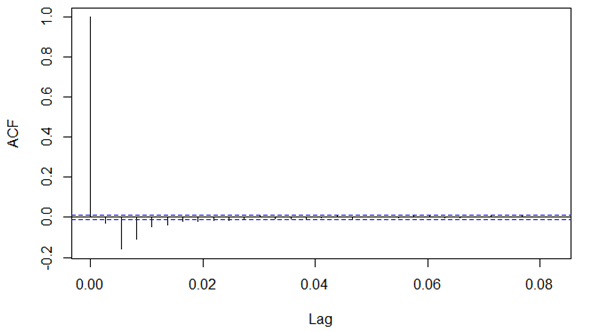
\includegraphics[width=0.7\textwidth]{images/part_1/autocorr3.png}
\end{figure}

\begin{figure}[H]
  \centering
    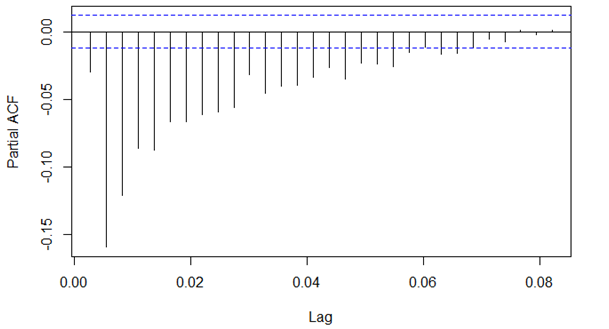
\includegraphics[width=0.7\textwidth]{images/part_1/autocorr4.png}
\end{figure}


\par On peut dès lors envisager de choisir $q = 6$. En revanche le choix de $p$ est problématique puisque la décroissance est très lente et les calculs sont trop lourds si l’on choisit $p = 21$ par exemple.

\par On peut ainsi considérer un modèle SARIMA365(26,1,6)(0,1,0). Néanmoins le temps de calcul est trop grand pour de telles valeurs, sans compter un risque important d’overfitting. On pressent que le tracé de autocorrélogramme partiel est pathologique, et un traitement plus important des données aurait été nécessaire afin d’obtenir une modélisation satisfaisante.
\end{document}